\section{Effective Action}

A minimal, consistent Lagrangian density implementing the ingredients above is
\begin{align}
 \mathcal{L}
 =\;& -\frac{\kappa_\omega}{4}\,\mathcal{W}^a_{\mu\nu}\,\mathcal{W}^{a\mu\nu}
 +\frac{\kappa_B}{12}\,H_{\mu\nu\rho}\,H^{\mu\nu\rho}
 +\frac{1}{2}(\nabla_\mu\Phi)(\nabla^\mu\Phi)-V(\Phi)
 +\frac{\theta}{4}\,\mathcal{W}^a_{\mu\nu}\,\tilde{\mathcal{W}}^{a\mu\nu} \nonumber\\
 &\;+\lambda_1\,(u_\mu u^\mu+1)\;+\;\lambda_2\,\nabla_\mu u^\mu
 +\sum_K \bar\Psi_K\!\left(i\gamma^\mu D_\mu - m_K^{(\mathrm{sol})}\right)\!\Psi_K ,
    \label{eq:EFT}
\end{align}
with
\[
    H_{\mu\nu\rho}\equiv \partial_{[\mu}B_{\nu\rho]},\qquad
    \tilde{\mathcal{W}}^{a\mu\nu}\equiv \tfrac{1}{2}\,\varepsilon^{\mu\nu\rho\sigma}\,\mathcal{W}^a_{\rho\sigma},\qquad
    D_\mu\equiv \nabla_\mu + i g_{\!sw}\,\mathcal{W}_\mu^a T^a .
\]
We adopt \(\varepsilon^{0123}=+1\) and the \((-+++)\) metric signature.
Here \(\nabla_\mu\) is the Levi–Civita (spin-)covariant derivative; on spinors it includes the spin connection.

\paragraph{Symmetries and constraints.}
The theory is invariant under
\(B\mapsto B+d\Lambda\) (2-form gauge) and local swirl-gauge transformations
\(\mathcal{W}_\mu \mapsto U^{-1}\!\big(\mathcal{W}_\mu + \tfrac{i}{g_{\!sw}}\partial_\mu\big)U\),
\(\Psi_K\mapsto U^{-1}\Psi_K\).
The Lagrange multipliers enforce a unit timelike condensate velocity and, if desired, covariant incompressibility \(\nabla_\mu u^\mu=0\).
The \(\theta\)-term \(\mathcal{W}\tilde{\mathcal{W}}\) is the non-Abelian Chern–Pontryagin density (a total derivative); in the present context it encodes helicity/knot-charge conservation.

\paragraph{Spinor fields as emergent quasiparticles.}
The Dirac term in \eqref{eq:EFT} provides the low-energy description of stabilized knotted swirl excitations labeled by a topological class \(K\) (e.g., torus knots). Their rest masses \(m_K^{(\mathrm{sol})}\) are non-perturbative soliton energies determined by the calibrated mass functional introduced later. The spinors transform under the swirl gauge group \(G_{\!sw}\) via \(D_\mu\).

\paragraph{Remarks.}
(i) No fundamental Yukawa couplings are introduced; fermion masses enter only through soliton energies.
(ii) Any gauge-boson screening/mass arises from medium effects (e.g., \(\Phi\)-dependent polarization) rather than SM-style Higgs couplings.
(iii) Appendix~\ref{sec:swirl-connection} outlines the coarse-grained origin of the swirl connection \(\mathcal{W}_\mu^a\).

\resizebox{\textwidth}{!}{%
    \centering
    \scriptsize
    \begin{figure}[h!]
        \centering
        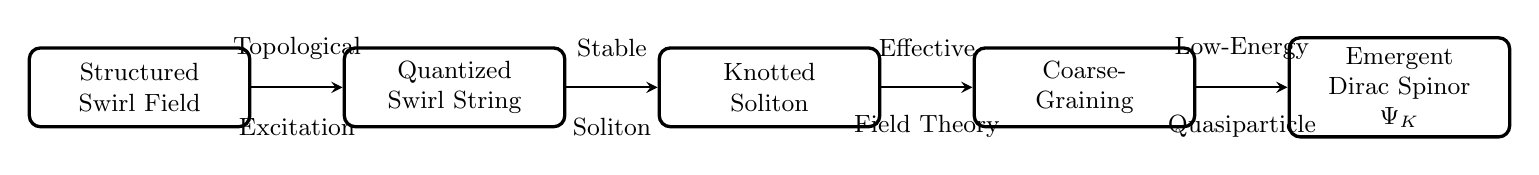
\begin{tikzpicture}[
            box/.style={rectangle, draw=black, very thick, rounded corners, minimum height=1cm, minimum width=2.8cm, align=center},
            arrow/.style={->, thick, >=stealth},
            every node/.style={font=\small}
        ]
            % Nodes
            \node[box] (condensate) at (0,0)  {Structured \\ Swirl Field};
            \node[box] (string)     at (4,0)  {Quantized \\ Swirl String};
            \node[box] (knot)       at (8,0)  {Knotted \\ Soliton};
            \node[box] (coarse)     at (12,0) {Coarse-\\Graining};
            \node[box] (dirac)      at (16,0) {Emergent \\ Dirac Spinor \\ $\Psi_K$};
            % Arrows
            \draw[arrow] (condensate) -- (string);
            \draw[arrow] (string) -- (knot);
            \draw[arrow] (knot) -- (coarse);
            \draw[arrow] (coarse) -- (dirac);
            % Labels
            \node at (2,0.5) {Topological};
            \node at (2,-0.5) {Excitation};
            \node at (6,0.5) {Stable};
            \node at (6,-0.5) {Soliton};
            \node at (10,0.5) {Effective};
            \node at (10,-0.5) {Field Theory};
            \node at (14,0.5) {Low-Energy};
            \node at (14,-0.5) {Quasiparticle};
        \end{tikzpicture}
        \caption{Emergence of effective spinor fields in Swirl-String Theory. Quantized swirl strings in a structured swirl condensate form knotted solitons which, under coarse-graining, behave as Dirac spinors in the EFT.}
        \label{fig:emergent-spinors}
    \end{figure}
}